\chapter{如何改善} % Introduction chapter suppressed from the table of contents

\hypertarget{ux67d0ux8f6fux4ef6ux5f00ux53d1ux516cux53f8ux654fux6377ux5f00ux53d1ux8fc7ux7a0bux6539ux8fdbux6848ux4f8b}{%
\subsection{敏捷开发过程改进案例}\label{ux67d0ux8f6fux4ef6ux5f00ux53d1ux516cux53f8ux654fux6377ux5f00ux53d1ux8fc7ux7a0bux6539ux8fdbux6848ux4f8b}}

\hypertarget{ux6708}{%
\subsubsection{5月}\label{ux6708}}

A公司一直专门为某电信公司提供针对客服、线上播放等服务服务。\\

张工是公司的中层管理者,管理好几个开发团队,有五位项目经理向他汇报。\\

他听说老同学的团队都开始用敏捷开发,很感兴趣,便参加了几次敏捷交流会,觉得可以解决很多开发团队的问题,尤其是可以快速交付给客户。\\

他便提建议给部门经理推动敏捷开发,找咨询公司做相关培训,例如 SCRUM Master 内部培训,然后全面开展实施。\\

开始时,部门经理有些怀疑,问:“听起来很吸引,但后面那些工程文档都不做,会不会影响质量和交付?客户都是专业做电信的,不缺钱,但是对质量要求很高。”\\

张工解释说,“只要利用敏捷把过程变成迭代,快速交付,改善工程的问题不难,主要是人的问题。”\\


部门经理听到敏捷可以比以前更快速交付,因之前客户经常抱怨项目延误,他也希望可以改变,就答应了。\\



\hypertarget{ux6708-1}{%
\subsubsection{8月}\label{ux6708-1}}

开发组长王工,三十出头,毕业后一直做开发,一年前晋升为组长。周五下班后与朋友喝酒,很开心地说:\\
“太兴奋了。我们团队刚参加了两天SCRUM 培训,并指出我们以前按传统瀑布式开发的种种问题。我们会2周一次迭代并割接上线,还会与用户代表定期交流,不再会像以前几个月交付后才发现开发出来的功能不合需求。\\
现在团队合作不像以前只按工种工作,也会跟产品经理、业务方面更充分合作,给客户带来更高价值。\\
工作方式也会改变,以前要写需求、规格说明书,现在简单化成用户故事和产品需求卡片,以前我们要做详细项目计划和甘特图。以后会改成用燃烧图和看板。 每天用便利贴去谢要开发什么东西贴在白板上面,我们会改成叫SCRUM Team。工作区周围都有SCRUM 的海报,提醒我们SCRUM的重点。我们也没项目经理了,自己管理自己。部门经理会变成产品负责人,敏捷开发方式让我们团队自己做决策,不仅仅是技术方面,项目相关的也由我们项目组一起讨论决定。”\\

\hypertarget{ux6708-2}{%
\subsubsection{9月}\label{ux6708-2}}

王工的朋友老杨周五晚喝酒时问王工:”你们团队学完敏捷SCRUM后,项目如何?”\\
王工立马面露笑容,充满自信地跟大家说:
``我们培训后就SCRUM的方法,定每两周一个冲刺,每次冲刺前都会用故事点来估算每个功能多大,然后按本次冲刺的资源,估计可以完成多少功能?
然后用看板来监控模块完成的情况,哪些在开发中,哪些已经完成,团队和管理者都可以一目了然,不用像以前......”\\
“听你这样说,我也要尽快提议领导引入敏捷开发。”\\
“我还未说完,我们每天早上也按照SCRUM的规定站立会议,每人说自己完成了哪些任务,今天做什么以前......”\\

\hypertarget{ux6708-3}{%
\subsubsection{10月}\label{ux6708-3}}

喝酒时老杨问王工:”你们项目如何?”\\
王工听完,没有立马回应,把注意力放在窗外的大街上,想了一下,然后说:
``我们本应上周要完成一次冲刺后的割接上线,但被推到下次了。``\\
''为什么?''\\
王工说:
''我们按培训学到的做冲刺计划会,按照产品的待办事项列表,团队利用扑克牌一起估算每一事项所需要的时间。我们总共八位开发人员,其中有一半是刚毕业不久,但大家刚上完培训,很有信心,虽然技术主管张工对我们出来的估算有些顾虑,觉得我们太理想,但大家刚培训完敏捷,张工也希望让部门经理尽快看到敏捷开发可以加快速度,我们就按这`进取式'估算开展2周冲刺。\\
但因新人多,编码水平有限,虽然大家已经尽快把开发出来的代码交给系统测试人员手工测试,依据测试发现的缺陷修正再测试,但割接上线期限前4天还是很多BUG没改好,最后3天,基本是天天加班,最终到上线期限仍然有不少问题,最终割接前测试,还是不能达到客户要求的水平,没办法,不能上线。

大家确实都尽力冲刺了,但未能达到我们本来希望的结果。``

“你们开发人员在提交代码到系统测试之前,有没有自己先自测?”

王工说:“我们敏捷开发每天早上站立会议上都用看板,记录每个模块的进度完成情况,开发编码人员都说自测过。”

“如果开发人员能自己把握好交付代码的质量。不应该等到系统测试才发现这么多问题要解决。你们团是怎么做自测?有记录吗?”

王工说:“这我就没有详细问了,因为我们学完SCRUM后,大家更关注开发速度,用看板保证按计划的进度,不延误。但没想到后面缺陷会这么多。而且有些问题改完以后还会导致另外一些BUG发生。到了最后,因为赶时间,大家对修改BUG已经麻木了。”

“你们之前不是都有代码评审和扫描的习惯吗?”

王工说:“之前,我们确实比较多评审,除了评审核心设计和代码,我们还要求组长抽查新人开发的代码,并且要求提交代码前必须通过扫描。但我们为加快速度,没有硬性要求必须先通过扫描。经你一问,我想这也可能是出现很多BUG的原因之一。”\\

“你们有没有事后迭代复盘?复盘可以帮团队分析之前有哪些不足,后面改进。”

王工说:“我们都交付不了,哪里有心情来做回顾、复盘。最后几天冲刺,大家每天都没睡好,大家都只想回去好好睡一觉。”


\hypertarget{ux6708-4}{%
\subsubsection{11月}\label{ux6708-4}}

部门经理之前收到客户总监电话,投诉一些技术缺陷,导致好几次不能按计划上线,问为什么正在交付的软件质量变差了?\\
张工被问到是什么原因时无法回答,只能说立马回去探索原因,尽快汇报\\

张工从部门经理办公室出来后,找其中一位项目经理李工喝茶,问他对今次敏捷改革的意见。\\

两人都赞同敏捷开发应能帮助团队提升,当张工问李工受什么可以改善的地方,李工说:“让团队自主是件好事,但因为我们专注做这块业务已经很多年了,本来业务的变化不多,只是一些功能小改动,所以开发人员尽量不去动核心代码,怕改动了反而会影响投产,切割不了。为了不动老代码,新代码都只能在核心的外围去写,但这种做法效率很低,不长久,估计一两年后会难以继续了,到时会被迫重写整个产品。而且懂老代码的开发人员大部分都离开了,代码维护越来越困难。

敏捷教练强调团队自主管理,给团队空间发挥。但SCRUM的教练缺乏软件工程的基础,只懂项目管理过程。所以他们也解决不了软件相关的问题。只是把精益管理怎么做迭代,怎么做回顾这些基本过程再解读一下,解决不了实际问题。”\\

张工说“很赞同,这是必须要解决的问题。但现在燃眉之急是要解决主管提出的客户投诉不能按时交付这紧急问题。不然我们以后也不敢再提敏捷开发了。”\\

无论张工或李工也没有能去总结出什么好的解决方案。现在推行敏捷才刚刚三个月,绝不能打退堂鼓,回到本来的状态。但应怎么解决敏捷带来的问题,挽回部门经理与客户的信心呢?
\begin{description}
\tightlist
\item[]
= = =
\end{description}

从上面的SCRUM案例看到,本来管理层希望利用敏捷开发,加快软件开发的交付,减少延误,令客户更满意。但因为只注重项目进度是否延误,但团队没注意如何改善软件开发本身的质量,也因为团队成员能力不足,开发出来的软件缺陷比以往还多,导致后面大量返工,恶性循环,后面更导致延误和客户投诉。\\
因为软件本身设计有问题,导致软件难以修改,开发人员都不敢改动任何代码,怕可能会引起系统崩溃。

怎样可以确保开发出来软件的质量?

敏捷开发有很多种方法(SCRUM
只是其一),因为目的不仅仅是管好项目进度,也要确保软件产品的质量。所以SCRUM
只包括项目管理部分,不全面。反过来,例如极限编程(XP eXtreme
Programming),因它的发明者Kent BECK
本身是一位精通面向对象的编程员,所以XP不仅仅关注项目管理,也包含编程的最佳实践。下图是
Ron Jeffery 把XP的重点画成从外到内3层:

%\href{文件:cleanagile_f1.8.jpg}{500px}。

\includegraphics[width=6cm]{cleanagile_f18.jpg}

SCRUM 只包含了外层的部分,缺乏中间和内层元素。
按XP的12实践(详见附件)都做到了便可以解决张工的问题吗?\\

\hypertarget{ux5982ux4f55ux6539ux5584}{%
\subsection{如何改善}\label{ux5982ux4f55ux6539ux5584}}

既然SCRUM方法有不足,XP方法能解决开发质量问题,是否团队学好XP便能帮助团队做好敏捷开发?\\
不一定,乔布斯离开苹果公司后,自己开创
NEXT,他接受访谈时总结了质量改进的重点:

\framebox{%
\begin{minipage}[t]{0.97\columnwidth}\raggedright
质量提升的道理其实很简单,是重复的过程:我们需要不断去看,有哪些无效的环节要省略,哪部分要重新设计,不断试验、提升,就这么简单。重点是所有的提升都应该是科学化的,有数据而不是泛泛而谈。

一般管理层的思路是:我是领袖,你们应该听我命令。但应该是反过来,让应如何做好的决定权利放在团队手上,做改进不需要请求管理层的批准。改进是工作的一部分,整个架构扁平化,自己管控日常过程,每位工程师应像以前的工匠,愿意花精力不断做好。然后能以自己最后做出的优质工艺、产物自豪。
\strut
\end{minipage}}

所以质量改进的原则:明确改进目标后不断完善的过程。这不仅仅适用于软件开发,也适用于其它,如工业生产用。

怎样才能不断完善,先问你以下关于汽车公司的问题:

%\href{文件:TvsGcompScreenshot_2023-06-07_121806.jpg}{650px}

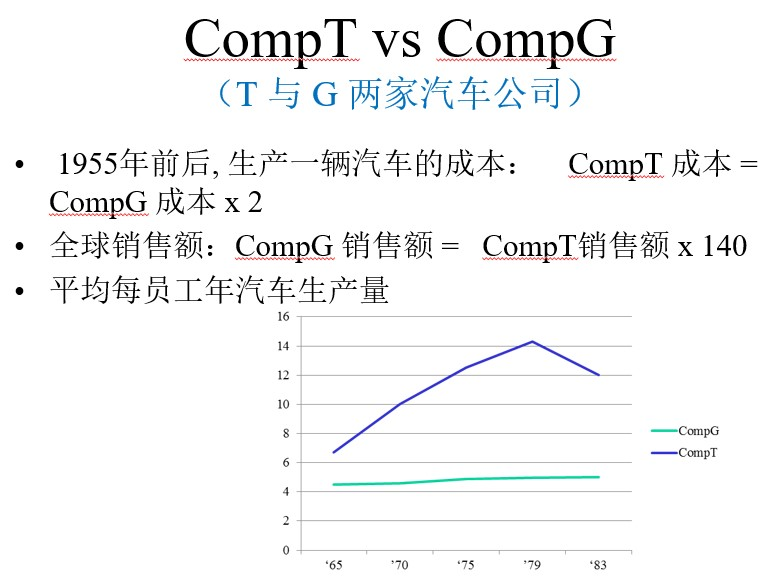
\includegraphics[width=6cm]{TvsGcompScreenshot_2023-06-07_121806.jpg}

T公司在六十年代,在销售、生产成本都远远不如G公司,但它每年生产率都一直提升。

请猜猜T和G是那家公司?
(提示:两家都是世界级汽车公司,现在你还能买到它们生产的汽车。)

\begin{description}
\item[]
\begin{description}
\tightlist
\item[]
= = = = = = = = = = = =
\end{description}
\end{description}

G 是美国通用; T 是日本丰田。

为什么丰田能从一家战后小公司能提升为世界最大 (\#) 的汽车公司?

\begin{description}
\item[]
\begin{description}
\tightlist
\item[]
(\# :
2023年底,总收入可能是大众第一,丰田第二,但丰田销售数量世界第一。)
\end{description}
\end{description}

\hypertarget{ux4e30ux7530ux6545ux4e8b}{%
\subsection{丰田故事}\label{ux4e30ux7530ux6545ux4e8b}}

\href{文件:ToyotaPresidentPicture1.png}{200px}\\
丰田喜一郎先生 (创始人)\\
%\href{文件:大野耐一.png}{200px}

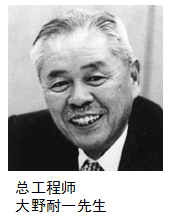
\includegraphics[width=6cm]{大野耐一.png}

二战后50年代,丰田汽车规模很小,经营很困难,在破产边缘。
但丰田创始人喜一郎先生明白美国生产线的弊端,意识到未来的汽车生产必须是Just-In-Time:

\begin{itemize}
\tightlist
\item
  每一辆都是按客人订单订制:例如,颜色,配置,左右钛等。
\item
  从钢材原料开始,整个生产线,零等待,零浪费。
\end{itemize}

\begin{description}
\item[]
\begin{description}
\tightlist
\item[]
每个工作步骤所需配件按生产需要到达
(不晚到也不早到),把生产过程中的配件降到零。
\end{description}
\end{description}

\url{文件:远景1.png}

喜一郎先生安排总工大野耐一去美国汽车公司考察。

\framebox{%
\begin{minipage}[t]{0.97\columnwidth}\raggedright
为什么福特Model-T 出名?它是第一辆一般人买得起的汽车
首辆现代汽车是由德国奔驰(Benz)于1885制作,
但是这些第一代汽车都非常昂贵。\\
老福特是一名工程师,对机械特别感兴趣,
白天是爱迪生公司的总工程师,到了下班后就研究汽车发动机
经过十年的不断优化,最终开发出4冲程(Quadcycle, a
self-propelled)自动汽车发动机 他的发明大大降低了汽车组件的成本 1908
Model-T 首次推出市场,售价是850美金,虽然已经比同期的其他厂家汽车便宜,
但还是超出一般工人家庭可以负担的水平。

为了进一步降低成本,老福特觉得必须想其他办法。
汽车组装一直都是作坊式运作, 所以组装汽车需要超过12个工时。
为了降低组装时间,必须要学其他工厂,
如啤酒,麦粉厂,它们都已经是流水式生产线生产(Assembly Line)
福特把整个Model-T组装拆分成84步骤, 并培训工人只做一项工作,
还聘用了科学工程师TAYLOR先生 设计整个流程,提高效率,
最终可以一个半小时完成组装一辆汽车。\\
生产线生产帮助福特公司把成本和售价降下来, 在15年期间(1913 -
1927),福特公司总共生产了15,000,000辆 Model-T。
虽然大量生产能直接降低生产成本, 但这种做法也要付出代价:

\begin{itemize}
\tightlist
\item
  为了生产所有都是同一个款式同一个颜色,黑色
\item
  为了提高生产的效率,也增加了组件的库存量
  (为了提高效率,降低成本,大部分组件都要批量生产(Batch
  production),例如轮胎。例如上面右下图看到工厂里存在大量轮胎。)
\end{itemize}

%\href{文件:FordModelT_2023-06-10_100431.jpg}{600px}

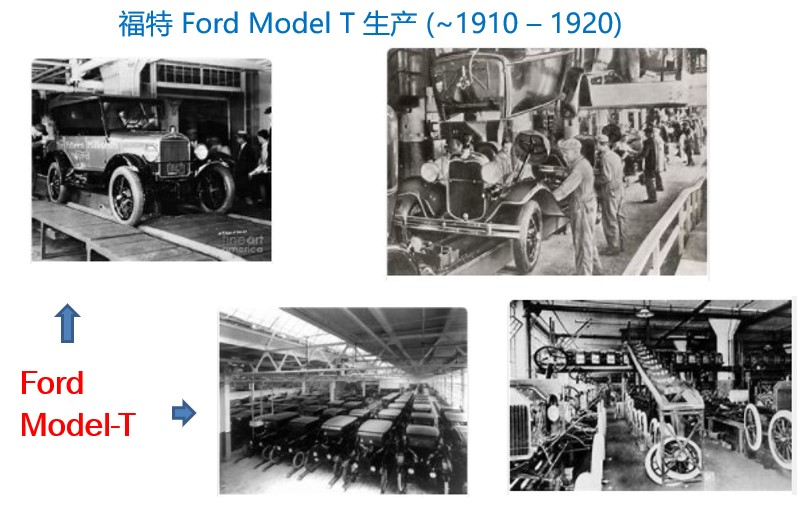
\includegraphics[width=6cm]{FordModelT_2023-06-10_100431.jpg}

\textbf{Federick TAYLOR与科学管理(Scientific Management)}\\
%\href{文件:Weisbord_P34.jpg}{200px}

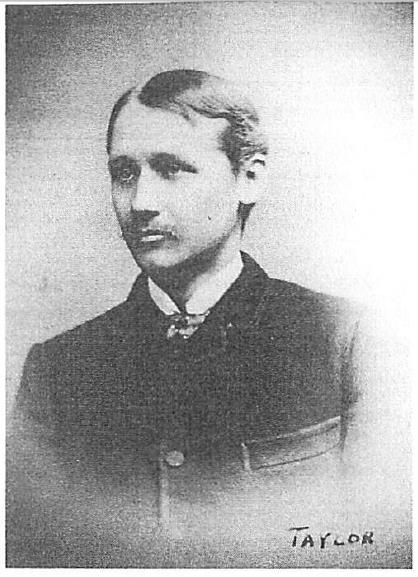
\includegraphics[width=6cm]{Weisbord_P34.jpg}

十九世纪末美国很多工业快速扩张,Taylor先生发现当时很多工厂生产力很低,例如钢铁厂。
他是很落地、实干的人,他就想有什么好方法可以让提高生产力,工人也多赚些钱。他发现很多工作都未设计好,未能好好利用工人,他针对工作本身做很多科学研究,测量每个工作应该多长时间,怎么做最好,然后按他的最佳设计把工作细分,也同时要求公司提高员工的奖励,希望工人看到因科学管理,提高生产,个人也受益。1890年,他加入了Bethlehem
Steel,钢铁业的大公司,帮它设计了很多奖励制度,也设定了一些叫工业工程师(Industrial
engineers)岗,发现生产力可以提升30-40\%。后来公司被收购,他也被辞退,他便成为顾问,当时都没有顾问这个职业,他可算是全球首位工程顾问。
\strut
\end{minipage}}

总工大野耐一先生,
从美国的超市(非汽车公司)得到如何做Just-In-Time的启发,回国后就开始在丰田致力推动。
开始时,很多人都觉得Just-In-Time 这个愿景好像是远不可及的梦想。

今天,现代汽车生产都基本做到了当年喜一郎先生和大野耐一先生的梦想。(详见附件)

\hypertarget{ux6c34ux9762ux4e0bux7684ux7ba1ux7406ux601dux8def}{%
\subsection{水面下的管理思路}\label{ux6c34ux9762ux4e0bux7684ux7ba1ux7406ux601dux8def}}

%\url{文件:冰山.png}

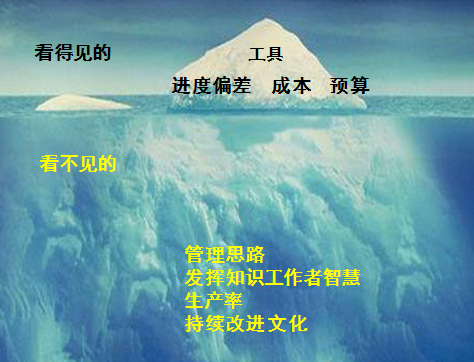
\includegraphics[width=6cm]{冰山.png}

为什么丰田能成功地把汽车生产做到 Just-In-Time
,超越西方的巨头,使日本汽车制造过程成为世界"标准"?
但我们不能单从表面看这"系统"的方法和技巧,例如大家都熟悉的看板管理(他的竞争对手通用、福特、肯定都学过),更重要是了解背后的管理思路。我们看看下面丰田九条原则,开始了解水面下的"系统":\\
\# 以忙碌为耻

\begin{enumerate}
\tightlist
\item
  培养人才 -- 逼他们动脑筋
\item
  从心里相信``大家的力量''
\item
  不以``我们公司''作主语
\item
  标杆管理
\item
  容易实现的目标不是好目标
\item
  根因分析
\item
  成长比成功更重要
\item
  所有人参与改进
\end{enumerate}

\hypertarget{ux4ee5ux5fd9ux788cux4e3aux803b}{%
\subsubsection{以忙碌为耻}\label{ux4ee5ux5fd9ux788cux4e3aux803b}}

\begin{itemize}
\tightlist
\item
  不吝惜智慧,但要吝惜汗水
\end{itemize}

\framebox{%
\begin{minipage}[t]{0.97\columnwidth}\raggedright
{把``动作''转变为 ``工作''}
以前,当大家批评某机关的工资太高时,职员会以上班时间很长,
``一直在努力工作''为由来反驳人们的批评。这其实是一种对于``有动作''和``在工作''的混淆。不管上班时间有多长,如果没能够创造出利润,那么就不能称之为工作,也不能称之为一直在努力。\\
丰田是把``动作''和``工作''分开考虑的。在丰田看来,
``就算一直在动也不代表那个人在工作''。
省掉徒劳动作,把``在动着''转化为``在工作''。\\大野耐一先生曾经问过年轻员工:
``每天工作一小时左右,你们能做到吗?"\\
听了这句话后,有人抱怨``算上加班时间,我们一天工作九个小时,他那句话是什么意思?"\\确实,他们在公司待了很长时间,但如果把``有动作''和``在工作''分开考虑,九个小时中,真正在工作的时间可能只有一小时。大野先生指的是这一点。\\ 关键的不在于流着汗在公司转了多长时间,而要把自己的工作区分成``徒劳作业''和``有价值作业''。
\strut
\end{minipage}}

因缺乏数据,很难判断这些软件开发人员每天有效生产多少?什么因素妨碍员工生产率提升?\\
\{\textbar{} class="wikitable" \textbar{}
二战后,日本经济萎缩,丰田辞退了不少员工。1950年,朝鲜战争,需要大量增产,但丰田选择了只增加设备,而不增加人手,大野先生也借这机会,完善丰田生产方式,成功找到了以不增加人手为前提的增产办法。

\textbar{}\}

\hypertarget{ux57f9ux517bux4ebaux624d---ux903cux4ed6ux4eecux52a8ux8111ux7b4b}{%
\subsubsection{培养人才 --
逼他们动脑筋}\label{ux57f9ux517bux4ebaux624d---ux903cux4ed6ux4eecux52a8ux8111ux7b4b}}

\framebox{%
\begin{minipage}[t]{0.97\columnwidth}\raggedright
{人了不起的智慧}
所谓丰田生产方式其实就是要建立起一种体制,把``人了不起的智慧''引导出来,使得这些智慧能在生产一线得到充分发挥。所以说``丰田生产方式源自人的智慧''。
\strut
\end{minipage}}

企业相信员工的智慧以后,员工们的干劲、使命感、责任感都会随之而生,最重要的是,员工们会因此逐渐对工作抱有自豪感。一旦员工们的意识改变了,理所当然地,企业的竞争力也将获得很大的提高。\\
丰田生产方式是TQM (Total Quality
Management全面质量管理)的最佳例子,TQM强调专注客户、持续改进、以数据说话、员工参与等,丰田生产方式覆盖了
TQM 原则的 七项 (除了战略)

%\href{文件:TQM_1.2.png}{500px}

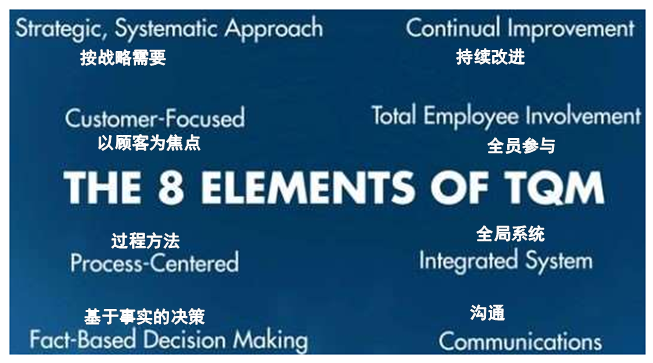
\includegraphics[width=6cm]{TQM_12.png}

\hypertarget{ux4eceux5fc3ux91ccux76f8ux4fe1ux5927ux5bb6ux7684ux529bux91cf}{%
\subsubsection{从心里相信``大家的力量''}\label{ux4eceux5fc3ux91ccux76f8ux4fe1ux5927ux5bb6ux7684ux529bux91cf}}

\begin{itemize}
\tightlist
\item
  不是靠``一个不平凡的人'',而是依靠``一百个平凡人''来创造亮眼的成绩。
\item
  生产产品就是培养人才。
\end{itemize}

\begin{description}
\tightlist
\item[]
``做事业最关键是人.......`培养人才'为基础''总裁丰田英二先生。
\end{description}

\begin{description}
\tightlist
\item[]
有一位丰田员工被问到``丰田生产方式到底是什么''的时候,这样回答:
``就是在人的智慧建起的基础上,立起了自动化和及时生产这两根支柱。''\\

\textbf{他所说的``人的智慧''是指``在一线工作人员的智慧''}。\\
\end{description}

\hypertarget{ux4e0dux4ee5ux6211ux4eecux516cux53f8ux4f5cux4e3bux8bed}{%
\subsubsection{不以``我们公司''作主语}\label{ux4e0dux4ee5ux6211ux4eecux516cux53f8ux4f5cux4e3bux8bed}}

\begin{itemize}
\tightlist
\item
  不是从``专业''的角度,而是从``顾客''的角度生产产品
\end{itemize}

\begin{description}
\tightlist
\item[]
创业大忌 --
闭门造车,所以丰田的原则,对客户有用就一定做出来,但对客户无用,或者不想要,就绝不生产。\\
\end{description}

%\url{文件:丰田p3.png}

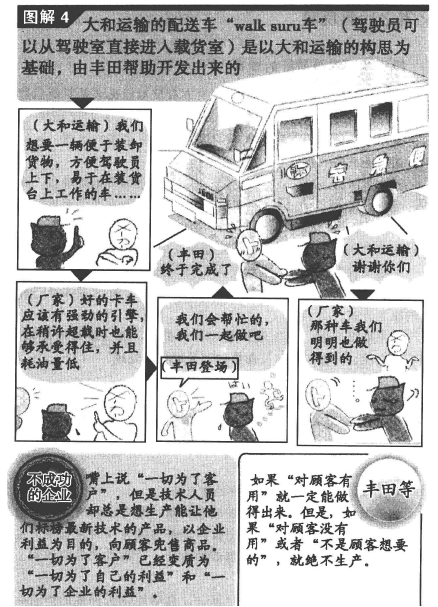
\includegraphics[width=6cm]{丰田p3.png}

要创新必须从``顾客''的角度看,不单从工程师的视角看不仅适用于丰田和汽车制造:

\framebox{%
\begin{minipage}[t]{0.97\columnwidth}\raggedright
征服太空,踏上月球。 六七十年代,美国开始阿波罗太空计划。
首批宇航员强烈要求工程师加上窗户、逃生门、可人手控制等
(现代我们会觉得这些是太空船 (spacecraft) 基本要求, 但当时是闻所未闻)

1980,一位NASA工程师回顾当时工程部的想法:
``你们又不是火箭专家,航天专家,只是飞行员。
希望可以在火箭驾驶舱人工控制火箭飞行,开玩笑!
太极端,你们可不了解成本多高,我们应可以很轻易用工程的理由拒绝。''
\strut
\end{minipage}}

\hypertarget{ux6807ux6746ux7ba1ux7406-benchmarking}{%
\subsubsection{标杆管理
(Benchmarking)}\label{ux6807ux6746ux7ba1ux7406-benchmarking}}

很多公司都会用百分比来设定改善目标,但改善了百分比,不一定代表质量有改善,例如
某快递公司去年送包裹未按时送达占8\%,今年是6\%,好像已经改善了2\%。
但去年托运的数量是500万件,所以8\%是4万件;
今年的数量是750万件,所以今年的6\%就是4万5千件。

所以今年包裹延误增加了5000,这样非但没有任何改善,反而服务变得更差了。所以更重要是看数字本身。容易达到的目标,不是好目标。所以丰田会一般选行业里最强的对手作为基准(标杆)。

1965年,美国通用汽车公司是世界顶尖。例如销售额的规模,丰田与通用是 1
: 60 完全不在同一个层次上

成本:丰田对通用是 1 : 0.5 成本是通用的一倍

丰田把当时顶尖的通用公司当成了自己进行标杆管理的对象

如果丰田某零件的成本价格是 1000日元,通用是400日元
丰田会把通用的400日元,作为基准成本价,把原料价定为400日元,把差额600作为``不必要花费'',让团队立马改善,尽早达到标杆。

丰田(如下图)很注重各种标杆,例如内部标杆、竞争性标杆等。软件开发也应该同样利用数据来制定量化目标。
%\url{文件:丰田p1.png}

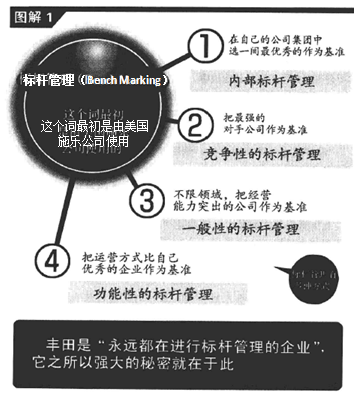
\includegraphics[width=6cm]{丰田p1.png}

\hypertarget{ux5bb9ux6613ux5b9eux73b0ux7684ux76eeux6807ux4e0dux662fux597dux76eeux6807}{%
\subsubsection{容易实现的目标不是好目标}\label{ux5bb9ux6613ux5b9eux73b0ux7684ux76eeux6807ux4e0dux662fux597dux76eeux6807}}

\begin{itemize}
\tightlist
\item
  不是``削减一成'',而是通过``取消一个零''来发现浪费
\end{itemize}

把原先需要三小时的工作,改用三分钟完成。\\
听到上司这个要求,你该怎么回答呢?多数人会常识性地回答:``这太强人所难了''、``绝对做不到''。\\

\framebox{%
\begin{minipage}[t]{0.97\columnwidth}\raggedright
丰田 \\
单分换模(Single Minute Exchange of
Die)''例子:\\ 1965年,丰田汽车在推行丰田生产方式时遭遇一个瓶颈:装置更换时间太长,其中特别是500吨冲压机和1000吨冲压机的模具,更换时间长达\\4小时。如果不缩短这两个模具的更换时间,就不可能实现多品种少量生产方式。\\ 挑战由大野耐一先生统领,在生产管理的先行者,新乡重夫先生的指导下,分两个阶段展开。\\
 改善开始之前,新乡先生凭借自己多年的工作经验,了解到装置更换有两种方式:\\
 ①内部装置更换------必须在机器停下来以后,才能进行的装置更换。\\
 ②外部装置更换------能在机器运转过程中,或是在运转起来以后,进行的装置更换。\\
 要缩短时间,把内部装置更换和外部装置更换清楚地分开来是一个关键。能在外部装置替换作业中进行的工作,就全部在外部装置替换过程中实施。同时,分别对内部装置替换和外部装置替换进行改善。通过这种方法,装置更换时间缩短为一个半小时。\\
 完成这一改善花费了半年时间。通常能有这样的成果就可以告一段落了。但是,大野先生仍要求进一步缩短时间。\\
 他要求把更换过程``缩短为3分钟!''通常通过改善能把原先的2\textasciitilde{}4小时缩短为一个半小时,就可以很满意地说``已经很好了''。但是,大野先生不这么想。
 他认为:
``既然能缩短到这个水平,那么继续改善肯定可以把时间缩短为3分钟。''
\\'''改变汽车生产的单分换模的秘密'''\\对于这一要求,在以新乡先生为中心的技术小组中,自然有人提出``3分钟绝对干不完''。但是,新乡先生认为:
``如果能把内部装置更换全部转化为外部装置更换,
3分钟也不是不可能......\\之后,他着手对多达100个以上的项目进行了改善。
\\ 首先,进一步对内部装置更换和外部装置更换进行细分,彻底把内部装置更换转化为外部装置更换。同时,想方设法对各种切割工具和模具进行设置,使得更换时用一个动作即可完成。此外,在紧固件上也动了很多脑筋。这样,终于创造出了无数项不花时间、能够简单完成同时可以在作业时保持稳定的改善。\\
紧接着,对作业顺序反复进行改善,实施标准化(制定没有多余工序的作业标准)。这样,在挑战进行了三个月后的某一天,真的只要3分钟就能完成了!这个结果让所有人都大吃一惊。
\strut
\end{minipage}}

\hypertarget{ux6839ux56e0ux5206ux6790}{%
\subsubsection{根因分析}\label{ux6839ux56e0ux5206ux6790}}

(五个为什么 是一种找根因的方法 , 详见附件B)

\begin{itemize}
\tightlist
\item
  不停留在``原因''上,而要找出``真因'',彻底改善。
\item
  不追究责任,而是追究原因。\\
\end{itemize}

丰田的大野耐一先生说:“做到一半是不行的,只有一个期限公司实施重建工作。当他第一天到达工厂的时候,他看到的是一副脏得无法形容的情景。机器上布满了油和灰尘,地板和墙壁上沾满污渍。飞散开来的机油上又落了灰尘,积成厚厚的一层。半成品和零件随便地东一堆西一堆地放着,工具扔得到处都是。工厂里想找块站的地方都很困难。这样的状态不用说也会降低丰田的“开动率”。仓库里也是堆满了零件和产品,但看那样子就知道,若要问起某个东西在哪里的话是不会有人知道的。

当工程师报了有问题就必须要求工程师查找原因、提供数据,但很多时候这个工作并不简单,但大野耐一先生决不放弃,必须找到根因。

\hypertarget{ux6210ux957fux6bd4ux6210ux529fux66f4ux91cdux8981}{%
\subsubsection{成长比成功更重要}\label{ux6210ux957fux6bd4ux6210ux529fux66f4ux91cdux8981}}

\begin{itemize}
\tightlist
\item
  要培养人才,``改变体制''比``改变人''更有效
\end{itemize}

有些工厂只依赖张贴标语、海报,希望可以减少工地的事故发生率,但丰田不注重喊口号,而是动手干实事,包括机械保安、设备保安等

%\href{文件:ft_223.1.png}{500px}

\includegraphics[width=6cm]{ft_2231.png}

所谓5S指的是:整理、整顿、清扫、清洁及修养。无法。。。产品的。。。。整顿''。实例:


\framebox{%
\begin{minipage}[t]{0.97\columnwidth}\raggedright
B 先生受命去子公司 A 公司实施重建工作。当他第一天到达工厂的时候,他看到的是一副脏得无法形容的情景。机器上布满了油和灰尘,地板和墙壁上沾满污渍。飞散开来的机油上又落了灰尘,积成厚厚的一层。半成品和零件随便地东一堆,西一堆地放着,工具扔得到处都是。工厂里想找块站的地方都很困难。这样的状态不用说也会降低丰田的“开动率”。仓库里也是堆满了零件和产品,但看那样子就知道,若要问起某个东西在哪里的话是不会有人知道的。\\

他在晨会上问大家: “你们想带自己的家人或恋人来这个工厂吗?”

A公司的员工们一直戒备着从总公司来的B先生新官上任后不知道会烧什么火,听到这句话后面面相觑。看来B先生好像对工厂的这个样子很不满意,他们一个个相视苦笑。就在大家不出声苦笑的过程中,不知道是谁轻轻说了一句“怎么可能带他们来呢”。声音虽然不大,但是B先生却没有漏听掉。“为什么不想带自己最亲近的人来看一看你们工作的地方呢?”“这么脏,哪好意思给人看啊。”“那为什么就让它一直这么脏着呢?”\\

这样追问以后,B先生听到了很多理由。“太忙了,没时间打扫”、“没有打扫的工具”、“没钱买重新粉刷的油漆”、“收拾好以后马上又脏了,扫了也是白搭”.....\\

心情”改变工作\\

在B先生听来,这些理由中其实就蕴含了“改善的线索”。\\

每当人们不想干什么事的时候,就会想出理由来辩解为什么干不了。大部分人都会因为这样的理由,而在是否要行动时犹豫再三。\\

但是, B先生身体力行丰田方式。他认为,找借口不如去思考该如何做。“用思考借口的脑袋来想怎么做”, “借口”其实和“之所以能做到的理由”是一致的。\\

B先生逐一攻破了A公司员工的“做不到的理由”。“没有时间”他就在工作时间中拿出几分钟将其设定为“清洁时间”。没有打扫工具和油漆,他就早早地买好。对于员工所说的“白搭”, B先生身先士卒地去捡垃圾、擦墙壁。\\

没过多久,原本很脏的工厂开始慢慢干净起来了。而当工厂开始变干净以后,员工们都产生了一种要把这种干净的状态维持下去的心情。他们开始自己收拾机器的漏油,而当初觉得“扫了也是白搭”的员工开始觉得“打扫也是件不坏的事”。\\

随着工厂开始变得干净起来,业绩也开始恢复了。工作的环境变好以后,在那里工作的人心情也就会随之出现了变化。


\strut
\end{minipage}}

大野耐一在他的《现场经营》中写过:

\framebox{%
\begin{minipage}[t]{0.97\columnwidth}\raggedright
如果仅仅觉得(机器人)用起来很方便,或是能代替我去工作,那就说明根本还没有能够有效地使用机器人。如果引进机器人,就要从引进的那一刻起对机器人进行改善,或者要使自己的做法能和机器人合拍。\\

如果公司老有人在嘀咕做这样的事买个机器人回来就成了,甚至在不明白目前的情况下有没有比引进机器人更好的方法,就成天想着如果不买机器人,改善就不可能进行得下去,那么,这家企业就糟糕了。首先要弄清楚目前企业里的机器能做到哪一步,或是为了使现在的机器能发挥更大的作用,而先充分地去使用现在的机器。这样当以后有先进的机器引进来的时候,就可以依靠其获得“基于智慧的+α’了。”丰田最终决定要在最后的组装工序中引进机器人也是经过了一段很长的准备期的。\\

比如说公司计划要把过去由自动机械完成的作业换成由机器人来完成。一般的做法无非就是直接用机器人把自动机械替换掉。但是,丰田首先挑选出典型的生产线,将这条生产线上原本由自动机械干的工作暂时换为人工作业。以此来详细地分析人会采用什么样的方法去做。并执行彻底的作业改善。在此基础上,探讨有什么工作是机器人做得了的,又有什么是机器人做不了的,以及为什么做不了。有的情况下还特意开发一些更容易能和机器人配合得起来的零件。他们是在经过了这样的过程以后,才和机器人的生产商共同开发,并最终决定导入机器人的。\\


实行机器人化并不是为了能够减少人数。在丰田不但“人的工作与机械(机器人)的工作”泾渭分明,而且两者的存在很和谐,推行机器人化是为了能让人去做附加值更高的工作。
\strut
\end{minipage}}

第一个例子,说明工作环境的重要性,主管通过逐步改善工厂的环境,团队的士气与生产率都提升了。

从第二个例子例子看到成长不是仅仅按既定方向做,必须思考动脑筋,并了解背后的目的才能真正取得效果。

这些丰田的成长故事也适用于软件开发团队,例如,有些软件开发团队盲目地想推自动化测试,却没有想好哪一类测试应自动化,哪一类更合适手工测试,最后因效果与投入不匹配,失败告终。

\hypertarget{ux6240ux6709ux4ebaux53c2ux4e0eux6539ux8fdb}{%
\subsubsection{所有人参与改进}\label{ux6240ux6709ux4ebaux53c2ux4e0eux6539ux8fdb}}

\framebox{%
\begin{minipage}[t]{0.97\columnwidth}\raggedright
{带诚意去赢得协作}
B先生所在的A公司曾以丰田生产方式为基础进行了生产改革。\\
 要进行生产改革没有技术部门的配合是行不通的。但是,任凭
B先生怎么要求,技术部门依然毫不合作。B先生实在没有办法了,只能向总裁要求:
``请加大我手上的权力,让我可以支配技术部。''总裁回答:
``你去给我请教了大野(耐一)先生以后再说!''\\
 于是B先生去找大野先生,在听他诉说了自己面临的窘境以后,大野先生对他说:
``你这一两天跟我一起去工厂转转吧!''并于百忙之中抽出时间带B先生参观了丰田的工厂以及附近的协作企业的工厂。这期间,大野先生什么话都没说,只在第二天下午问B先生:``怎么样,你明白了吗?''\\
 B先生回答:
``我觉得在工厂听到的关于厂长的改善事例,跟丰田方式所强调的重点好像不太一致。''听了B先生的回答以后,大野先生点头:
``就连我,也是一直都在忍耐的啊。工作并不是有权力就能解决问题的。要想得到对方的理解和信任,拿出诚意去找人家吧。''\\
 从那以后,
B先生再也不找``因为我手里没有权力''之类的借口,而总是带着诚意去找对方协商,不久以后,他成功地对A公司实施了生产改革。\\
 每当听到有人感慨``下属不听话''的时候,一位曾在丰田工作的人就会说:
``你要求自己的孩子"每天学习三小时'时,他会听话去学习吗?''\\
 对方的回答是:
``估计没用。''\\
 ``连自己的孩子都这样,更何况那些成年的员工呢?''
\strut
\end{minipage}}

\hypertarget{ux6539ux5584ux8d28ux91cf}{%
\subsection{改善质量}\label{ux6539ux5584ux8d28ux91cf}}

质量管理,与财务管理类似,同样也有质量策划、质量控制和质量改进,基于这大框架再细分:如何制定质量目标,如何来制定度量等。\\
质量策划包括:

\begin{enumerate}
\tightlist
\item
  设定目标,包括外部和内部目标。
\item
  识别内部需求。
\item
  依据客户需求制定产品的功能特征。
\item
  制定产品和过程的目标。
\item
  设计过程来达到这些目标,最后验证过程能力。\\
\end{enumerate}

\textbf{质量控制和质量改进}\\
下图的左面是在过程之前的策划部分,例如发现缺陷比率为20\%,这就是过程的能力,这是策划的时候已经定好的,过程控制没有什么可以做,只是当缺陷有变化,比如特别高的时候,需要做一些措施返回本来的水平。例如希望把缺陷从20\%降到3\%,这就必须驱动一系列的改进计划。改进计划也必须按项目管理方法推行与监控,没有其它办法。\\
%\href{文件:JuranImprovementScreenshot_2022-10-23_211444.jpg}{500px}

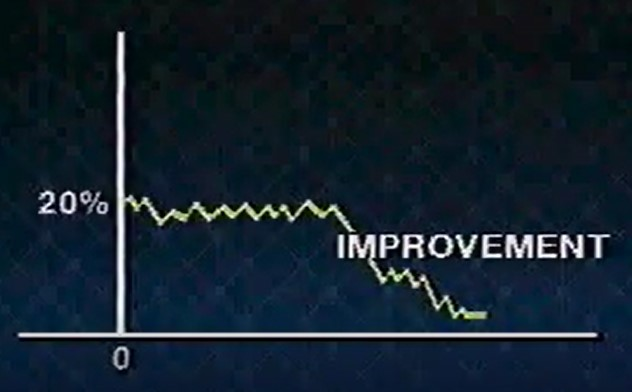
\includegraphics[width=6cm]{JuranImprovementScreenshot_2022-10-23_211444.jpg}\\

所以如果希望利用敏捷开发,不仅仅是走迭代,确保进度没偏差,还要确保软件产品质量,也应该用裘兰博士的质量管理思路去看敏捷过程,才能更全面了解如何才可以确保软件开发的质量,也控制好交付工期、不延误,让客户满意。\\
最佳实践,如果没有定质量目标,配上度量衡量和策划,都只是空想,对长远提升公司文化、团队成员的习惯没有任何帮助。举例:参照上图,例如我们想改善团队的策划和估算。首先要识别客户,哪些是主要干系人
-
甲方有什么要求;内部部门经理,有什么要求。然后从他们的诉求变成过程的功能和特征,但如果特征只是描述,没有数字也没有意义,所以要配合可衡量的度量单位,和用什么方式去收集那些数字,然后依据目标定过程要怎么去做,怎样改。

不是单纯”空降”某敏捷流程(例如 SCRUM),便能加快团队的发布速度。
所以虽然极限编程里每一条实践都是最佳实践,也必须配合质量策划,和监控改进才会有效果。

\hypertarget{ux7ed3ux675fux8bed}{%
\subsection{结束语}\label{ux7ed3ux675fux8bed}}

虽然XP比SCRUM更全面列出敏捷团队的最佳实践,但还必须依赖团队持续改善才会有效果。
从丰田故事看到``系统''如何帮公司培养知识工作者,发挥人的无限智慧,
为公司增值。\\
汽车制造大部分利用自动化机器,但当今软件开发生产和质量,
非常依赖开发人员的水平, 所以我们更需要建立``系统'',帮助员工快速成长。

前面分享的九个丰田管理思路:

\begin{enumerate}
\tightlist
\item
  以忙碌为耻
\item
  培养人才 -- 逼他们动脑筋
\item
  从心里相信``大家的力量''
\item
  不以``我们公司''作主语
\item
  标杆管理 
\item
  容易实现的目标不是好目标
\item
  根因分析
\item
  成长比成功更重要
\item
  所有人参与改进
\end{enumerate}

丰田汽车,从50年代开始,沿用裘兰博士 (Dr
JURAN)的质量管理思路,成为世界最大的汽车企业。

针对软件开发,如何基于以上质量管理、精益管理思路,配合敏捷开发最佳实践,提升产品质量与团队竞争力?

所以团队成员,包括团队组长与组员,的能力是过程改进的基础,不仅仅依赖领导人。

按质量大师裘兰博士定义,质量包括两部分:

\begin{itemize}
\tightlist
\item
  满足客户需要 (包括外部客户和内部客户)
\item
  没有缺陷\\
\end{itemize}

这定义不仅仅适合于制造业,也适用于服务业、IT业。\\
因软件开发团队都有缺陷管理系统记录缺陷数,我们主要讨论如何降低后期暴露的缺陷,让客户更满意的过程改进方法。例如在第五部分会详细说明如何做好量化迭代回顾,降低验收测试和系统测试的缺陷密度。

下一部分,我们探索`团队与自我改善基本功' 与成功要素。

\hypertarget{ux9644ux4ef6}{%
\section{附件}\label{ux9644ux4ef6}}

\hypertarget{ux73b0ux4ee3ux6c7dux8f66ux751fux4ea7}{%
\subsection{现代汽车生产}\label{ux73b0ux4ee3ux6c7dux8f66ux751fux4ea7}}

今天Just-In-Time已成为汽车制造的主流,例如:日产在英国牛津(Oxfordshire)专门生产mini
车的 工厂便能做到:

\begin{itemize}
\tightlist
\item
  从钢材原料到生产出汽车只需要24小时。
\item
  整个生产线没有任何中间等候,每68秒出一辆。
\item
  每天生产1000辆车。
\end{itemize}

%\href{文件:NissanRobots-OIP.h8UAC7FBjlaCmA_mBepJjQHaEi.jpg}{500px}\\
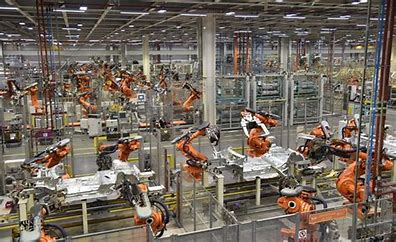
\includegraphics[width=6cm]{NissanRobots-OIPh8UAC7FBjlaCmA_mBepJjQHaEi.jpg}\\
\textbf{挑战}:每一辆汽车都不同 -- 颜色、设备、左右驾驶座等

\begin{itemize}
\tightlist
\item
  生产线上每一辆汽车都按照客户需求订制。
\item
  组件不早不晚按需求准时到达生产线。
\item
  这便需要信息化系统把客户订单转换成生产信息。
\end{itemize}

%\href{文件:NissanJIT_OIP.RQGKy67DWGTu-DQiOCqW2gHaEK.jpg}{500px}
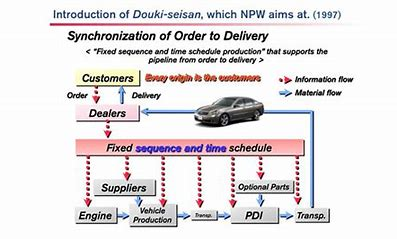
\includegraphics[width=6cm]{NissanJIT_OIPRQGKy67DWGTu-DQiOCqW2gHaEK.jpg}\\

例如,生产线上每一辆的颜色都可以不同:\\
%\href{文件:NissanProdLineOIP.wJFmfMl7q2_V8JaQi4kQ8QHaE6.jpg}{400px}\\
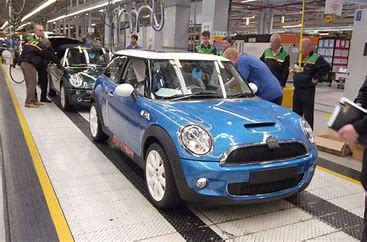
\includegraphics[width=6cm]{NissanProdLineOIPwJFmfMl7q2_V8JaQi4kQ8QHaE6.jpg}\\

\hypertarget{xp}{%
\subsection{XP}\label{xp}}

\hypertarget{ux7f16ux7801ux5b9eux8df5-coding-practices}{%
\subsubsection{编码实践 Coding
Practices}\label{ux7f16ux7801ux5b9eux8df5-coding-practices}}

\hypertarget{cp1ux7b80ux5355ux5730ux7f16ux7801ux548cux8bbeux8ba1-code-and-design-simply}{%
\paragraph{CP1:简单地编码和设计 Code and Design
Simply}\label{cp1ux7b80ux5355ux5730ux7f16ux7801ux548cux8bbeux8ba1-code-and-design-simply}}

\begin{itemize}
\tightlist
\item
  To produce software that is easy to change 使软件易于更改
\end{itemize}

\hypertarget{cp2ux65e0ux60c5ux5730ux91cdux6784-refactor-mercilessly}{%
\paragraph{CP2:无情地重构 Refactor
Mercilessly}\label{cp2ux65e0ux60c5ux5730ux91cdux6784-refactor-mercilessly}}

\begin{itemize}
\tightlist
\item
  To find the code's optimal design 找到代码的最佳设计
\end{itemize}

\hypertarget{cp3ux5236ux5b9aux7f16ux7801ux6807ux51c6-develop-coding-standards}{%
\paragraph{CP3:制定编码标准 Develop Coding
Standards}\label{cp3ux5236ux5b9aux7f16ux7801ux6807ux51c6-develop-coding-standards}}

\begin{itemize}
\tightlist
\item
  To communicate ideas clearly through code 通过代码清晰地传达想法
\end{itemize}

\hypertarget{cp4ux5171ux540cux7684ux8bcdux6c47-develop-a-common-vocabulary}{%
\paragraph{CP4:共同的词汇 Develop a Common
Vocabulary}\label{cp4ux5171ux540cux7684ux8bcdux6c47-develop-a-common-vocabulary}}

\begin{itemize}
\tightlist
\item
  To communicate ideas about code clearly 清楚传达软件设计的想法
\end{itemize}

\hypertarget{ux5f00ux53d1ux5b9eux8df5-develop-practices}{%
\subsubsection{开发实践 Develop
Practices}\label{ux5f00ux53d1ux5b9eux8df5-develop-practices}}

\hypertarget{dp1ux6d4bux8bd5ux9a71ux52a8ux5f00ux53d1tdd-test-driven-development}{%
\paragraph{DP1:测试驱动开发TDD
Test-Driven-Development}\label{dp1ux6d4bux8bd5ux9a71ux52a8ux5f00ux53d1tdd-test-driven-development}}

\begin{itemize}
\tightlist
\item
  To prove that code works as it should 来证明软件正常工作:\\
\end{itemize}

\begin{description}
\tightlist
\item[]
- Test-first programming(prim practice\#)
\end{description}

\hypertarget{dp2ux7ed3ux5bf9ux7f16ux7a0b-pair-programming}{%
\paragraph{DP2:结对编程 Pair
Programming}\label{dp2ux7ed3ux5bf9ux7f16ux7a0b-pair-programming}}

\begin{itemize}
\tightlist
\item
  To spread knowledge, experience and ideas 传播知识、经验和想法:\\
\end{itemize}

\begin{description}
\tightlist
\item[]
- Pair Programming(prim practice\#)
\end{description}

\hypertarget{dp3ux96c6ux4f53ux8d1fux8d23ux5199ux597dux4ee3ux7801vs-ux53eaux987eux8651ux81eaux5df1ux7684ux4ee3ux7801-collective-code-ownership-vs-individual-own-code}{%
\paragraph{DP3:集体负责写好代码(vs 只顾虑自己的代码) Collective Code
Ownership (vs individual own
code)}\label{dp3ux96c6ux4f53ux8d1fux8d23ux5199ux597dux4ee3ux7801vs-ux53eaux987eux8651ux81eaux5df1ux7684ux4ee3ux7801-collective-code-ownership-vs-individual-own-code}}

\begin{itemize}
\tightlist
\item
  To spread the responsibility for the code to the whole team
  将写好代码的责任扩展到整个团队:\\
\end{itemize}

\begin{description}
\tightlist
\item[]
- Whole team(prim practice\#)

- Share code(corollary practice\#)
\end{description}

\hypertarget{dp4ux6301ux7eedux96c6ux6210-integrate-continually}{%
\paragraph{DP4:持续集成 Integrate
Continually}\label{dp4ux6301ux7eedux96c6ux6210-integrate-continually}}

\begin{itemize}
\tightlist
\item
  To reduce the impact of adding new features 降低添加新功能的影响:
\end{itemize}

\begin{description}
\tightlist
\item[]
- Incremental Design(prim practice\#)

- Single code base(corollary practice\#)

- Ten-minute Build(prim practice\#)

- Continuous Integration(prim practice\#)
\end{description}

\hypertarget{ux5546ux52a1ux5b9eux8df5-business-practices}{%
\subsubsection{商务实践 Business
Practices}\label{ux5546ux52a1ux5b9eux8df5-business-practices}}

\hypertarget{bp1ux5c06ux5ba2ux6237ux6dfbux52a0ux8fdbux56e2ux961f-add-a-customer-to-the-team}{%
\paragraph{BP1:将客户添加进团队 Add a Customer to the
Team}\label{bp1ux5c06ux5ba2ux6237ux6dfbux52a0ux8fdbux56e2ux961f-add-a-customer-to-the-team}}

\begin{itemize}
\tightlist
\item
  To address business concerns accurately and directly
  准确、直接地解决业务问题:
\end{itemize}

\begin{description}
\tightlist
\item[]
- Real Customer involvement(corollary practice\#)
\end{description}

\hypertarget{bp2ux8ba1ux5212ux6e38ux620f-play-the-planning-game}{%
\paragraph{BP2:计划游戏 Play the Planning
Game}\label{bp2ux8ba1ux5212ux6e38ux620f-play-the-planning-game}}

\begin{itemize}
\tightlist
\item
  To schedule the most important work 安排最重要的工作:\\
\end{itemize}

\begin{description}
\tightlist
\item[]
- Weekly cycle ; Quarterly cycle ; Slack (prim practice\#)
\end{description}

\hypertarget{bp3ux5b9aux671fux53d1ux5e03-release-regularly}{%
\paragraph{BP3:定期发布 Release
Regularly}\label{bp3ux5b9aux671fux53d1ux5e03-release-regularly}}

\begin{itemize}
\tightlist
\item
  To return the customer's investment often
  尽早交付,让客户看到投资回报:
\end{itemize}

\begin{description}
\tightlist
\item[]
- Incremental Deployment(corollary practice\#)

- Daily Deployment(corollary practice\#)
\end{description}

\hypertarget{bp4ux4ee5ux53efux6301ux4e45ux7684ux901fux5ea6ux5de5ux4f5c-work-at-a-sustainable-pace}{%
\paragraph{BP4:以可持久的速度工作 Work at a Sustainable
Pace}\label{bp4ux4ee5ux53efux6301ux4e45ux7684ux901fux5ea6ux5de5ux4f5c-work-at-a-sustainable-pace}}

\begin{itemize}
\tightlist
\item
  To go home tired, but not exhausted 回家时虽然很累,但不筋疲力尽:\\
\end{itemize}

\begin{description}
\tightlist
\item[]
- Slack (prim practice\#)
\end{description}

\hypertarget{sux6cd5}{%
\subsection{5S法}\label{sux6cd5}}

本来5S是用于工业生产,例如日本的生产工厂很注重洁净,东西要放在容易找到的固定位置。其实这对生产线员工有很重要的心理作用。如果整个环境都很脏,必然会影响人工做好的动力,如果东西乱放,也容易找不到。5S也不仅仅是用于生产,医院、酒店也采用这方式管理,每件东西必须放在固定位置;这也可以用于个人管理,我以前常常在出差去客户现场时,经常忘记把一些东西,如鼠标或插头。但后面我固定了每件东西都应放哪里,临走收拾时就确保那些东西不会遗漏掉。平常工作有一个洁净的环境,也能降低工作压力,提高工作效率。\\

\href{文件:5S_五常法_Screenshot_2023-08-03_211606.jpg}{400px}

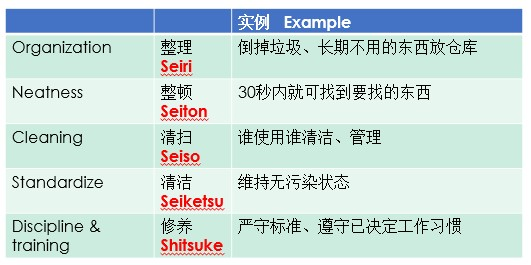
\includegraphics[width=6cm]{5S_五常法_Screenshot_2023-08-03_211606.jpg}\\

\hypertarget{ux53c2ux8003-references}{%
\section{参考 References}\label{ux53c2ux8003-references}}

\begin{enumerate}
\tightlist
\item
  若松义人, 《为什么是丰田:成为第一的方法和7个习惯》
\end{enumerate}


